\pagebreak
\subsection{Sequence Diagram}

\paragraph[]{Sequence diagram for traditional product entity update.} \hspace{1mm} \par
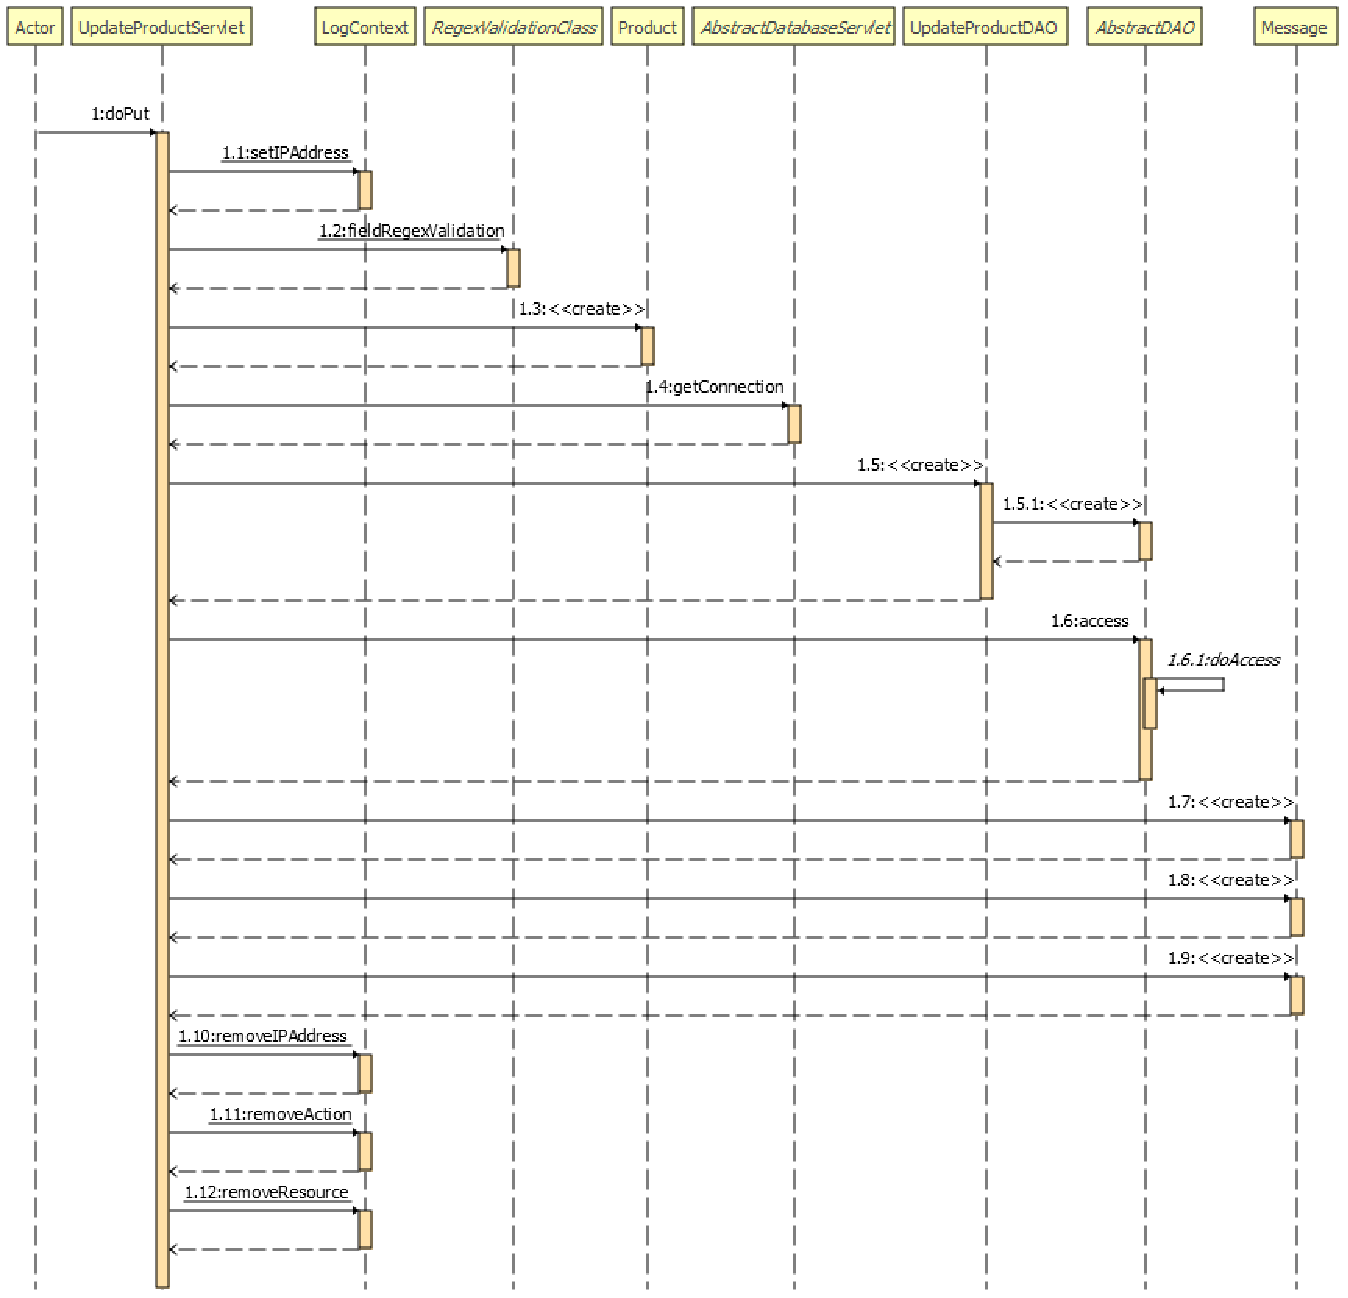
\includegraphics[width=\textwidth, keepaspectratio]{resources/updateproductsequence.pdf}
In the schema above is shown the sequence diagram for the update of a product (servlet + DAO). 

The user sends a PUT request to the web server. The web server calls the UpdateProductServlet and then sets the IP address of LogContext and also checks, using the class regex validation, that the parameters passed in input are valid.

Then a new object of class Product is created, with the parameters passed in input. After this, the UpdateProductServlet calls the getConection() method of the AbstractDatabaseServlet. After doing this, the servlet instantiate a new object of the class UpdateProductDAO, which extends AbstractDAO (so an object of AbstractDAO is created).

Then, with the doAccess() method of the class AbstractDAO, the DAO connects to the database.

After connecting to the database and executing the SQL statement, three messages for the servlet are created.

Finally, the resources are removed for the clean-up.
\pagebreak
\paragraph[]{Sequence diagram for rest get customer resource.} \hspace{1mm} \par
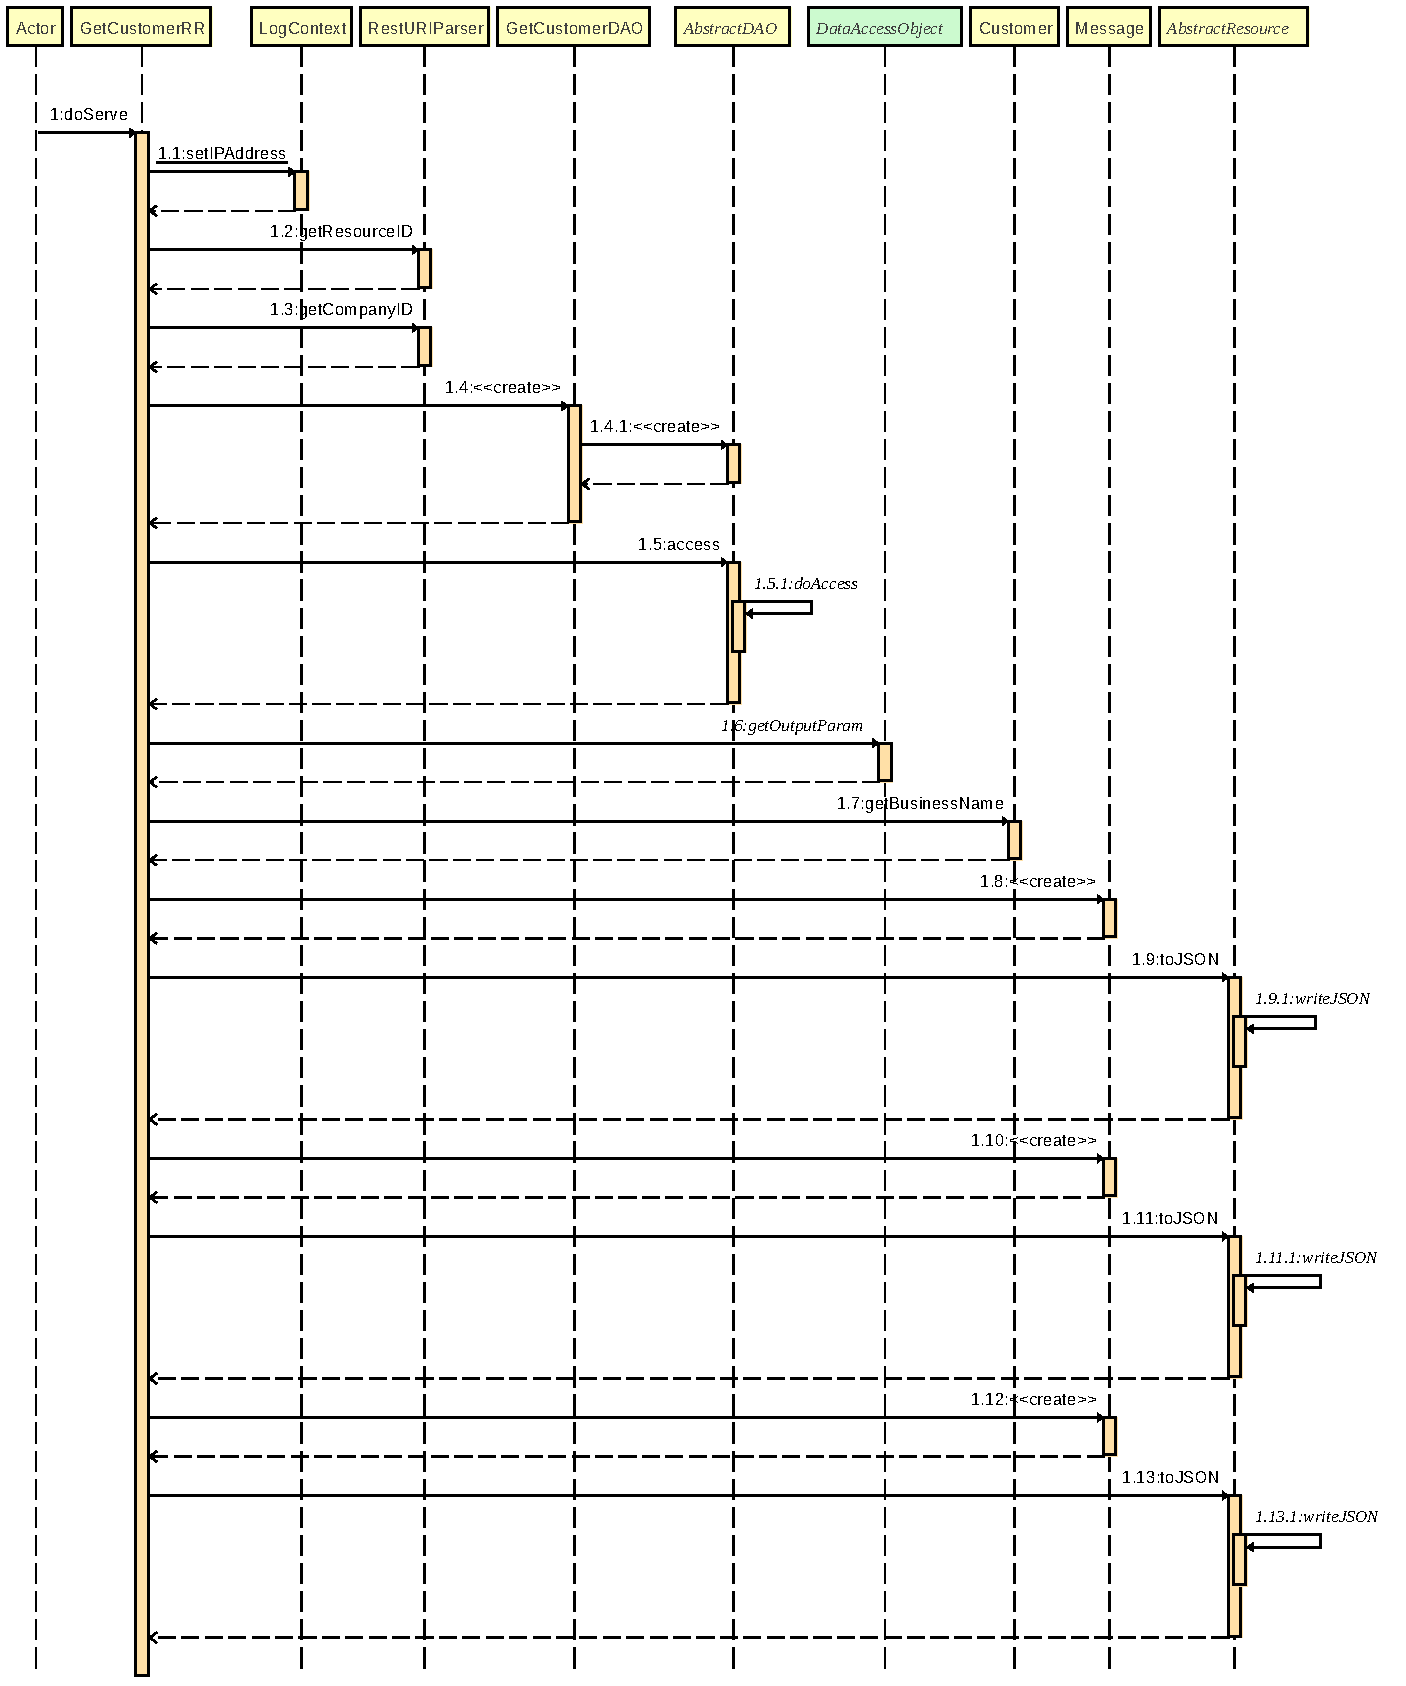
\includegraphics[width=\textwidth, keepaspectratio]{resources/getcustomersequence.pdf}
In the schema above is shown the sequence diagram for the get of a customer (rest resource + DAO). 

The user sends a GET request to the web server, which analyzes the request and calls the GetCustomerRR. This class the setIPAddress() of the LogContext and then retrieves the URI parameters with the getResourceID() and getCopanyID() of the RestURIParser class.

After having the parameters stored, an instance of the class GetCustomerDAO is created by the rest resource, and also an instance of AbstractDAO is created, because the GetCustomerDAO extends AbstractDAO. The DAO accesses the database with the doAccess() method, and retrieves the customer.

The servlet calls the getOutputParam() method of the DataAccessObject class and gets the output parameters asked by the user. An instance of the Customer class is retrieved and, with the getBusinessName() method, the servlet gets the business name of the customer retrieved.

After doing all of this, three messages are created and, with the toJSON() method of the AbstractResopurce class, a JSON with the data of these messages are written (with writeJSON()). The content of this messages is based on the results of the GET request.